\documentclass[11pt,a4paper]{article}

% -------------------------------------------------
% Required packages
% -------------------------------------------------
\usepackage[margin=1in]{geometry}
\usepackage[table,dvipsnames]{xcolor}

% -------------------------------------------------
% Colors (defined BEFORE tikz and hyperref)
% -------------------------------------------------
\definecolor{certiblue}{RGB}{37,99,235}
\definecolor{certigreen}{RGB}{5,150,105}
\definecolor{certired}{RGB}{220,38,38}
\definecolor{certipurple}{RGB}{124,58,237}
\definecolor{certidark}{RGB}{15,23,42}
\definecolor{certigray}{RGB}{100,116,139}
\definecolor{attackblue}{RGB}{219,234,254}
\definecolor{attackgreen}{RGB}{220,252,231}
\definecolor{attackorange}{RGB}{255,237,213}
\definecolor{attackred}{RGB}{254,226,226}
\definecolor{attackpurple}{RGB}{243,232,255}
\definecolor{codebg}{RGB}{248,250,252}

\usepackage{tikz}
\usetikzlibrary{shapes.geometric,arrows.meta,positioning,fit,backgrounds,calc}
\usepackage{booktabs}
\usepackage{tabularx}
\usepackage{listings}
\usepackage[most]{tcolorbox}
\usepackage{fancyhdr}
\usepackage{titlesec}
\usepackage[T1]{fontenc}
\usepackage[utf8]{inputenc}
\usepackage{lmodern}
\usepackage{amsmath,amssymb}
\usepackage{multirow}
\usepackage{array}
\usepackage{float}
\usepackage{caption}
\usepackage{enumitem}
\usepackage[colorlinks=true,linkcolor=certiblue,citecolor=certiblue,urlcolor=certiblue]{hyperref}

% -------------------------------------------------
% Page style
% -------------------------------------------------
\pagestyle{fancy}
\fancyhf{}
\fancyhead[L]{\textcolor{certidark}{\small\textbf{CertiGuard SDK --- Architecture Document}}}
\fancyfoot[C]{\thepage}
\renewcommand{\headrulewidth}{0.4pt}
\renewcommand{\footrulewidth}{0pt}

% -------------------------------------------------
% Section styling
% -------------------------------------------------
\titleformat{\section}
{\Large\bfseries\color{certiblue}}
{\thesection}{0.7em}{}
[\vspace{0.2em}\color{certiblue}\titlerule]

\titleformat{\subsection}
{\large\bfseries\color{certidark}}
{\thesubsection}{0.6em}{}

\titleformat{\subsubsection}
{\normalsize\bfseries\color{certidark}}
{\thesubsubsection}{0.6em}{}

% -------------------------------------------------
% Listings style
% -------------------------------------------------
\lstdefinestyle{certicode}{
  backgroundcolor=\color{codebg},
  basicstyle=\ttfamily\small,
  keywordstyle=\color{certiblue}\bfseries,
  commentstyle=\color{certigray}\itshape,
  stringstyle=\color{certigreen},
  numbers=left,
  numberstyle=\tiny\color{certigray},
  numbersep=8pt,
  frame=single,
  framerule=0.3pt,
  rulecolor=\color{certigray},
  breaklines=true,
  showstringspaces=false
}
\lstset{style=certicode}

% -------------------------------------------------
% tcolorbox style
% -------------------------------------------------
\tcbset{
  certicallout/.style={
    colback=white,
    colframe=certiblue,
    boxrule=0pt,
    borderline west={2.5pt}{0pt}{certiblue},
    arc=2pt,
    left=8pt,
    right=8pt,
    top=6pt,
    bottom=6pt
  }
}

% -------------------------------------------------
% Helpers
% -------------------------------------------------
\newcolumntype{Y}{>{\raggedright\arraybackslash}X}
\setlist[itemize]{leftmargin=1.4em,itemsep=0.3em}
\setlist[enumerate]{leftmargin=1.6em,itemsep=0.3em}

\begin{document}

% =================================================
% SECTION 1: Title Page
% =================================================
\begin{titlepage}
\centering
\vspace*{1.2cm}

{\Huge\bfseries\color{certiblue}CertiGuard SDK\par}
\vspace{0.35cm}
{\Large\color{certidark}On-Premise Software License Protection\par}
\vspace{0.2cm}
{\large\color{certipurple}\textbf{Defense-in-Depth: A 10-Layer Architecture}\par}

\vspace{0.8cm}
{\normalsize\color{certigray}\textbf{Prevention $\cdot$ Detection $\cdot$ Forensics $\cdot$ Offline-First}\par}
\vspace{0.25cm}
{\normalsize\color{certigray}InnovIA ESI Hackathon --- April 2026\par}

\vspace{1.0cm}

\begin{figure}[H]
\centering
\begin{tikzpicture}[node distance=0.08cm]
  \foreach \i/\name/\c in {
    10/Audit Log \& Evidence Chain/certipurple,
    9/Watermarking \& Attribution/certipurple,
    8/Behavioral AI Detection/certigreen,
    7/Honeypot Tripwires/certigreen,
    6/PoW Dead Man's Switch/certigreen,
    5/Anti-Debug \& Anti-Tamper/certigreen,
    4/Challenge-Response Verifier/certiblue,
    3/Installation DNA \& Counter/certiblue,
    2/Hardware Fingerprint/certiblue,
    1/Ed25519 Signature Core/certiblue
  }{
    \node[draw=\c, fill=\c!18, rounded corners=2pt, minimum width=10.8cm, minimum height=0.7cm, anchor=north] (L\i) at (0,{-0.8*(10-\i)}) {\textbf{L\i}: \name};
  }
\end{tikzpicture}
\caption{CertiGuard 10-layer vertical defense stack}
\end{figure}

\vfill
{\small\color{certigray}Software Architecture Design Document (SADD) --- IEEE-style technical format\par}
\end{titlepage}

\tableofcontents
\newpage

% =================================================
% SECTION 2
% =================================================
\section{System Overview}

\subsection{The Problem}
On-premise software is frequently attacked through license-file editing, debugger-assisted binary patching, virtual-machine cloning, and usage abuse. Traditional single-check licensing fails because attackers need to bypass only one gate. CertiGuard addresses this with a layered architecture where cryptographic trust, host binding, runtime verification, behavioral detection, and forensic evidence are chained into one offline-first control plane.

\subsection{Why Existing Solutions Fail}
\begin{table}[H]
\centering
\caption{Limitations of common licensing approaches}
\begin{tabularx}{\textwidth}{>{\bfseries}lY}
\toprule
Existing approach & Why it fails in practice \\
\midrule
Plain serial key check & Static key checks are patched by flipping a branch instruction in minutes. \\
Online-only activation & Air-gapped or restricted enterprise networks cannot depend on real-time cloud checks. \\
Simple hardware lock & Single-factor hardware binding is bypassed by VM snapshots or partial spoofing. \\
Code obfuscation only & Obfuscation raises effort but does not provide cryptographic authenticity or evidence trail. \\
Periodic polling license server & ``Kill server, keep app running'' attack remains possible without local heartbeat enforcement. \\
\bottomrule
\end{tabularx}
\end{table}

\subsection{CertiGuard's Approach}
CertiGuard implements a defense-in-depth model: signed license authenticity (L1), machine/installation context continuity (L2--L3), verifier challenge integrity (L4), anti-analysis and liveness controls (L5--L6), tamper tripwires (L7), local anomaly scoring (L8), leak attribution (L9), and immutable audit chaining (L10). The system remains operational offline while preserving post-event forensic visibility for vendor review.

\begin{figure}[H]
\centering
\begin{tikzpicture}[
  node distance=1.1cm and 1.3cm,
  >=Latex,
  server/.style={draw=certidark, fill=white, rounded corners, minimum width=3.2cm, minimum height=2.1cm, align=center},
  file/.style={draw=certigray, fill=white, minimum width=2.2cm, minimum height=1.0cm, align=center},
  shield/.style={draw=certiblue, fill=certiblue!20, minimum width=2.3cm, minimum height=2.3cm, regular polygon, regular polygon sides=6, align=center},
  atk/.style={->, very thick, certired},
  ok/.style={->, very thick, certiblue}
]
\node[server] (client) {Client Application\\\small Runtime + SDK};
\node[file, right=1.8cm of client] (lic) {License\\\texttt{.certiguard}};
\node[shield, below=0.9cm of $(client)!0.5!(lic)$] (shield) {\textbf{CertiGuard}\\Shield};

\draw[ok] (lic.west) -- (client.east) node[midway, above, sloped, text=certiblue] {\small verified flow};

\node[left=2.6cm of client, text=certired] (a1) {\small File editing};
\node[left=2.6cm of $(client.south west)+(0,-0.6)$, text=certired] (a2) {\small License copy};
\node[above=1.3cm of client, text=certired] (a3) {\small Debug attach};
\node[above=1.3cm of lic, text=certired] (a4) {\small VM clone};
\node[right=2.4cm of lic, text=certired] (a5) {\small Snapshot rollback};
\node[below=1.5cm of lic, text=certired] (a6) {\small Over-usage};

\draw[atk] (a1.east) -- ($(shield.west)+(-0.05,0.35)$);
\draw[atk] (a2.east) -- ($(shield.west)+(-0.05,-0.35)$);
\draw[atk] (a3.south) -- ($(shield.north)+(-0.35,0.05)$);
\draw[atk] (a4.south) -- ($(shield.north)+(0.35,0.05)$);
\draw[atk] (a5.west) -- ($(shield.east)+(0.05,0.1)$);
\draw[atk] (a6.north) -- ($(shield.south)+(0.2,-0.05)$);
\end{tikzpicture}
\caption{The attack surface and CertiGuard shielded runtime}
\end{figure}

% =================================================
% SECTION 3
% =================================================
\section{Architecture Layers}

\subsection{Layered Design Diagram}
\begin{figure}[H]
\centering
\begin{tikzpicture}[>=Latex, node distance=0.08cm]
% Left labels
\node[anchor=east, text=certiblue, font=\bfseries] at (-0.55,7.45) {PREVENTION};
\node[anchor=east, text=certigreen, font=\bfseries] at (-0.55,4.05) {DETECTION};
\node[anchor=east, text=certipurple, font=\bfseries] at (-0.55,1.6) {FORENSICS};

\foreach \idx/\y/\name/\desc/\col in {
1/7.2/Ed25519 Signing/Core authenticity of license payload/certiblue,
2/6.45/Hardware Fingerprint/Bind license to host hardware profile/certiblue,
3/5.7/Installation DNA/Detect clone and rollback continuity breaks/certiblue,
4/4.95/Separate Verifier/Challenge-response integrity verification/certiblue,
5/4.2/Anti-Debug/Detect active runtime reverse engineering/certigreen,
6/3.45/Dead Man's Switch/PoW heartbeat chain enforces liveness/certigreen,
7/2.7/Honeypot Fields/Tripwire keys catch payload edits/certigreen,
8/1.95/Behavioral AI/Isolation Forest flags abusive patterns/certigreen,
9/1.2/Watermarking/Per-customer encoded attribution signal/certipurple,
10/0.45/Audit Hash Chain/Tamper-evident forensic event ledger/certipurple
}{
  \node[draw=\col, fill=\col!15, rounded corners=2pt, minimum width=13.0cm, minimum height=0.62cm, anchor=west] (bar\idx) at (0,\y) {};
  \node[draw=\col, fill=\col, text=white, circle, minimum size=0.52cm, anchor=west] at (0.18,\y) {\small\textbf{\idx}};
  \node[anchor=west, font=\bfseries, text=certidark] at (0.88,\y+0.12) {\name};
  \node[anchor=west, text=certigray] at (0.88,\y-0.12) {\small \desc};
}
\end{tikzpicture}
\caption{CertiGuard prevention--detection--forensics layer stack}
\end{figure}

\subsection{Complete Layer Catalogue}
\begin{table}[H]
\centering
\caption{Layer model, threat focus, and offline suitability}
\small
\begin{tabularx}{\textwidth}{c l Y Y c}
\toprule
\textbf{Layer} & \textbf{Name} & \textbf{Threat Stopped} & \textbf{Algorithm/Method} & \textbf{Offline?} \\
\midrule
L1 & Ed25519 Signing & File tampering, forgery & EdDSA on Curve25519 & YES \\
L2 & Hardware Fingerprint & License copying & SHA-256 + CPU/Board & YES \\
L3 & Installation DNA & VM cloning, snapshots & UUID + Timestamp + Counter & YES \\
L4 & Separate Verifier & Binary patching & Challenge-response HMAC & YES \\
L5 & Anti-Debug & Debugger analysis & IsDebuggerPresent + timing + ptrace & YES \\
L6 & Dead Man's Switch & Process killing & PoW heartbeat chain & YES \\
L7 & Honeypot Fields & License editing & Tripwire fields in payload & YES \\
L8 & Behavioral AI & Over-usage, sharing & Isolation Forest (sklearn) & YES \\
L9 & Watermarking & Leak tracing & Per-customer encoding & YES \\
L10 & Audit Log & Evidence destruction & SHA-256 hash chain & YES \\
\bottomrule
\end{tabularx}
\end{table}

\begin{tcolorbox}[certicallout,title=\textbf{Design Principle}]
No single layer is trusted as a sole control. Runtime acceptance requires a sequence of independent controls whose outputs are both \emph{decision signals} and \emph{forensic events}.
\end{tcolorbox}

% =================================================
% SECTION 4
% =================================================
\section{Data Flow Diagram}

\begin{figure}[H]
\centering
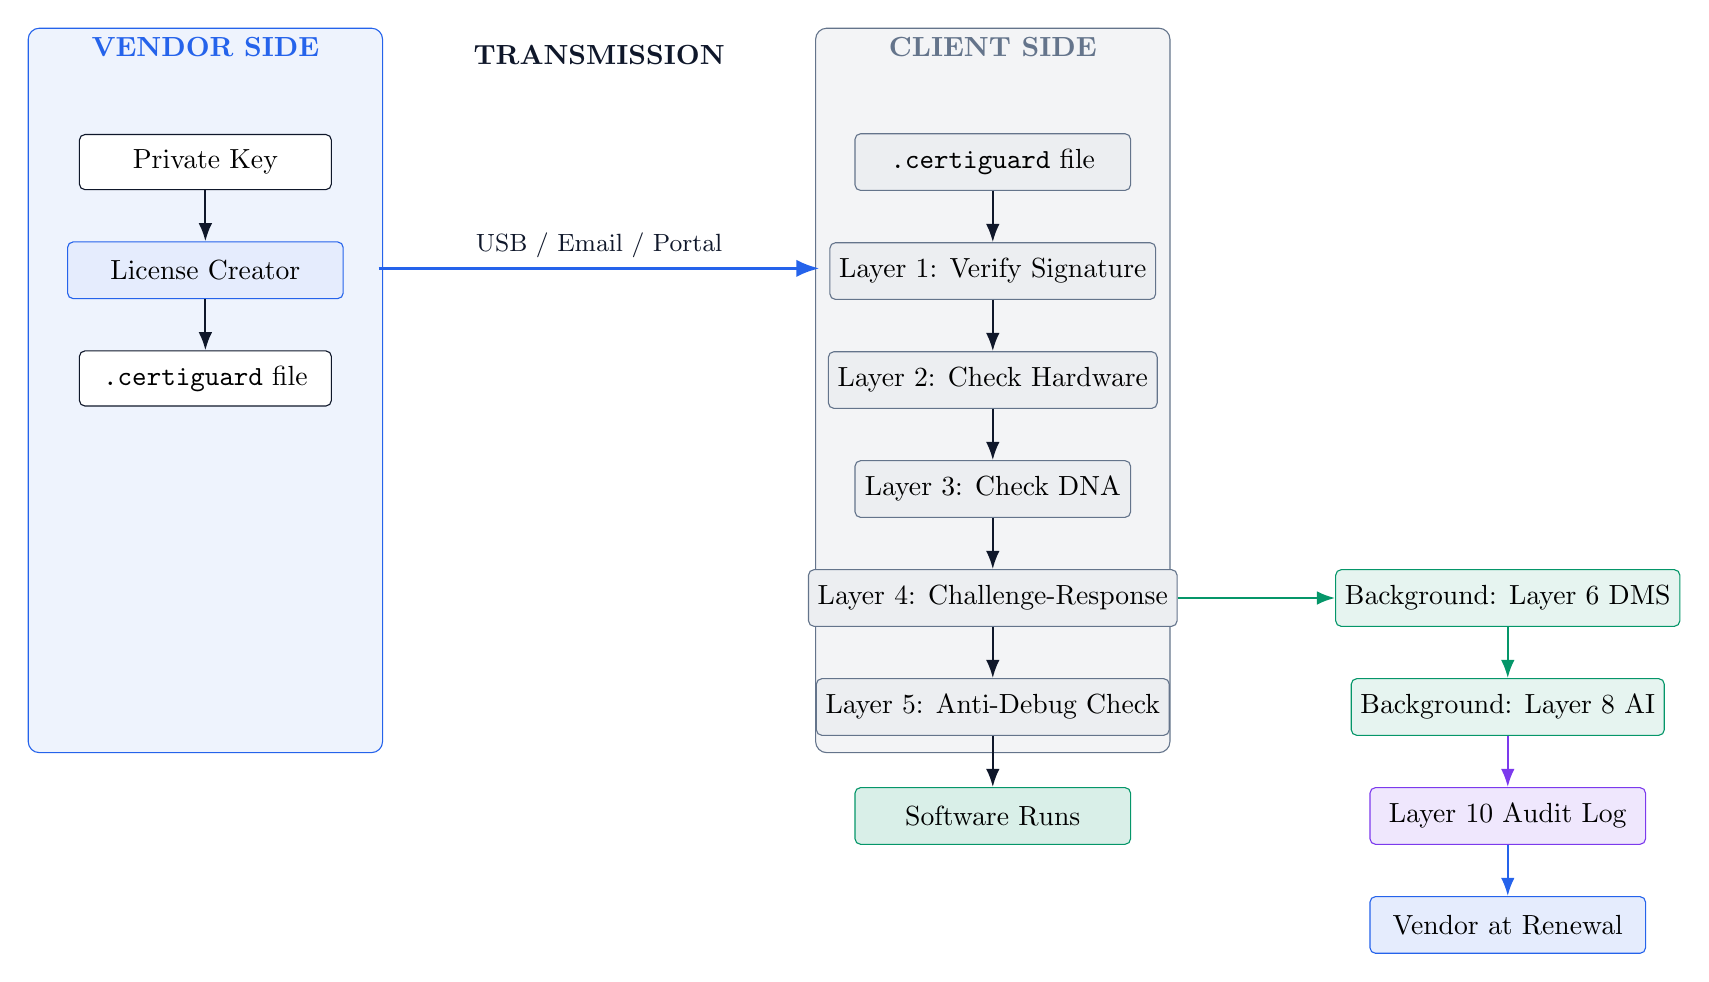
\begin{tikzpicture}[
  >=Latex,
  node distance=0.65cm and 1.35cm,
  box/.style={draw=certidark, rounded corners=2pt, fill=white, minimum width=3.2cm, minimum height=0.7cm, align=center},
  proc/.style={draw=certiblue, rounded corners=2pt, fill=certiblue!12, minimum width=3.5cm, minimum height=0.72cm, align=center},
  side/.style={draw=certigray, rounded corners=2pt, fill=certigray!12, minimum width=3.5cm, minimum height=0.72cm, align=center},
  arr/.style={->, thick, certidark}
]

% Column backgrounds
\node[draw=certiblue, fill=certiblue!8, rounded corners, minimum width=4.5cm, minimum height=9.2cm] (vendorbg) at (-5.0,0.0) {};
\node[draw=certigray, fill=certigray!8, rounded corners, minimum width=4.5cm, minimum height=9.2cm] (clientbg) at (5.0,0.0) {};

\node[anchor=north, text=certiblue, font=\bfseries] at (vendorbg.north) {VENDOR SIDE};
\node[anchor=north, text=certigray, font=\bfseries] at (clientbg.north) {CLIENT SIDE};
\node[anchor=north, text=certidark, font=\bfseries] at (0,4.5) {TRANSMISSION};

% Vendor chain
\node[box] (k) at (-5.0,2.9) {Private Key};
\node[proc, below=of k] (lc) {License Creator};
\node[box, below=of lc] (licv) {\texttt{.certiguard} file};

\draw[arr] (k) -- (lc);
\draw[arr] (lc) -- (licv);

% Transmission arrow
\draw[->, very thick, certiblue] (-2.8,1.55) -- (2.8,1.55)
node[midway, above, text=certidark] {\small USB / Email / Portal};

% Client chain
\node[side] (licc) at (5.0,2.9) {\texttt{.certiguard} file};
\node[side, below=of licc] (l1) {Layer 1: Verify Signature};
\node[side, below=of l1] (l2) {Layer 2: Check Hardware};
\node[side, below=of l2] (l3) {Layer 3: Check DNA};
\node[side, below=of l3] (l4) {Layer 4: Challenge-Response};
\node[side, below=of l4] (l5) {Layer 5: Anti-Debug Check};
\node[draw=certigreen, fill=certigreen!15, rounded corners=2pt, minimum width=3.5cm, minimum height=0.72cm, align=center, below=of l5] (run) {Software Runs};

\draw[arr] (licc) -- (l1);
\draw[arr] (l1) -- (l2);
\draw[arr] (l2) -- (l3);
\draw[arr] (l3) -- (l4);
\draw[arr] (l4) -- (l5);
\draw[arr] (l5) -- (run);

% Parallel background branch
\node[draw=certigreen, fill=certigreen!10, rounded corners=2pt, minimum width=3.5cm, minimum height=0.72cm, align=center, right=2.0cm of l4] (dms) {Background: Layer 6 DMS};
\node[draw=certigreen, fill=certigreen!10, rounded corners=2pt, minimum width=3.5cm, minimum height=0.72cm, align=center, below=of dms] (ai) {Background: Layer 8 AI};
\node[draw=certipurple, fill=certipurple!12, rounded corners=2pt, minimum width=3.5cm, minimum height=0.72cm, align=center, below=of ai] (audit) {Layer 10 Audit Log};
\node[draw=certiblue, fill=certiblue!12, rounded corners=2pt, minimum width=3.5cm, minimum height=0.72cm, align=center, below=of audit] (renewal) {Vendor at Renewal};

\draw[->, thick, certigreen] (l4.east) -- (dms.west);
\draw[->, thick, certigreen] (dms) -- (ai);
\draw[->, thick, certipurple] (ai) -- (audit);
\draw[->, thick, certiblue] (audit) -- (renewal);
\end{tikzpicture}
\caption{End-to-end vendor-to-client data and control flow}
\end{figure}

% =================================================
% SECTION 5
% =================================================
\section{Ed25519 Cryptographic Core}

\subsection{Mathematical Foundation}
CertiGuard's trust anchor is vendor-side Ed25519 signing. The client validates signatures using only the public key.

\begin{align*}
\text{Private key:}\quad & d = \texttt{random\_bytes}(32) \\
\text{Public key:}\quad & Q = d \cdot G \\
\text{Signature:}\quad & \sigma = (R,S), \quad S = (r + k\cdot d)\bmod L \\
\text{Verification:}\quad & S\cdot G = R + k\cdot Q
\end{align*}

\begin{tcolorbox}[certicallout,title=\textbf{Security Implication}]
Without the vendor private key $d$, a valid signature over a modified license payload is computationally infeasible under standard Ed25519 assumptions.
\end{tcolorbox}

\subsection{Why This Beats Denuvo-Style Decrypt-at-Runtime Patterns}
\begin{table}[H]
\centering
\caption{Comparison: code decryption DRM vs signed-parameter architecture}
\begin{tabularx}{\textwidth}{>{\bfseries}lYY}
\toprule
Property & Denuvo DRM & CertiGuard \\
\midrule
What's protected & Game executable code & License parameters and policy payload \\
Secret in RAM? & YES --- decryption key material is transiently present & NO --- private key remains vendor-side only \\
Dump attack? & Possible via runtime memory dump during decrypt path & Not applicable; no private signing key in client runtime \\
Status & Historically cracked in multiple titles & Signature forgery remains mathematically infeasible \\
\bottomrule
\end{tabularx}
\end{table}

\subsection{License File Structure}
\begin{lstlisting}[language=,caption={Conceptual signed license payload (all fields covered by signature)}]
{
  "version": "3.0",
  "license_id": "LIC-20260425025054",
  "issued_to": "Customer A",
  "issued_at": "2026-04-25T02:50:54Z",
  "valid_until": "2027-04-25T02:50:54Z",
  "hardware_fingerprint": "sha256(...)",
  "install_dna": {
    "install_id": "uuid-v4",
    "first_boot": "2026-04-01T10:00:00Z",
    "boot_count_at_issue": 37
  },
  "parameters": {
    "max_users": 50,
    "modules": ["core", "analytics"]
  },
  "tpm": {
    "available": true,
    "anchor": "optional-tpm-anchor"
  },
  "watermark": "customer-bound-short-hash",
  "tripwires": {
    "premium_unlock": false,
    "admin_override": false
  }
}
\end{lstlisting}

% =================================================
% SECTION 6
% =================================================
\section{Installation DNA --- Anti-Cloning}

\subsection{The VM Cloning Problem}
A cloned VM can preserve application files, including the license file, but cannot preserve all runtime continuity signals simultaneously. CertiGuard combines machine-bound encryption context, first-boot chronology, and monotonic counters to make state replay and snapshot rollback observable.

\subsection{Three DNA Components}
\begin{figure}[H]
\centering
\begin{tikzpicture}
\node[anchor=west, font=\bfseries, text=certidark] at (0,3.2) {Component};
\node[anchor=west, font=\bfseries, text=certidark] at (4.2,3.2) {Original VM};
\node[anchor=west, font=\bfseries, text=certidark] at (8.4,3.2) {Clone after snapshot};
\node[anchor=west, font=\bfseries, text=certidark] at (13.1,3.2) {Result};

\draw[certigray] (0,3.0) -- (16.2,3.0);

\foreach \c/\ov/\cv/\r/\y in {
UUID/a3f9.../Cannot decrypt (wrong HW)/REJECTED/2.35,
First-Boot/2026-04-01/2026-04-15 (new boot)/MISMATCH/1.6,
Boot Counter/150/100 (went backward)/REJECTED/0.85
}{
  \node[anchor=west, text=certidark] at (0,\y) {\c};
  \node[anchor=west, text=certidark] at (4.2,\y) {\ov};
  \node[anchor=west, text=certidark] at (8.4,\y) {\cv};
  \node[anchor=west, text=certired, font=\bfseries] at (13.1,\y) {\r};
  \draw[certigray!45] (0,\y-0.25) -- (16.2,\y-0.25);
}
\draw[certigray!60] (3.7,0.5) -- (3.7,3.0);
\draw[certigray!60] (8.0,0.5) -- (8.0,3.0);
\draw[certigray!60] (12.7,0.5) -- (12.7,3.0);
\end{tikzpicture}
\caption{DNA continuity checks under VM clone/snapshot conditions}
\end{figure}

\subsection{Why All Three Cannot Be Cloned Simultaneously}
A successful clone attack would require simultaneously reproducing (i) hardware-derived cryptographic context, (ii) installation timeline consistency, and (iii) monotonic counter progression. In practical enterprise environments, attackers can imitate one or two signals, but not all three without triggering at least one mismatch event and corresponding forensic evidence.

% =================================================
% SECTION 7
% =================================================
\section{AI Behavioral Detection}

\subsection{Isolation Forest --- How It Works}
Isolation Forest isolates anomalous points using random partition trees; observations requiring fewer splits are more likely to be outliers. CertiGuard applies this locally on runtime usage features and persists baseline statistics to support offline enforcement.

\begin{figure}[H]
\centering
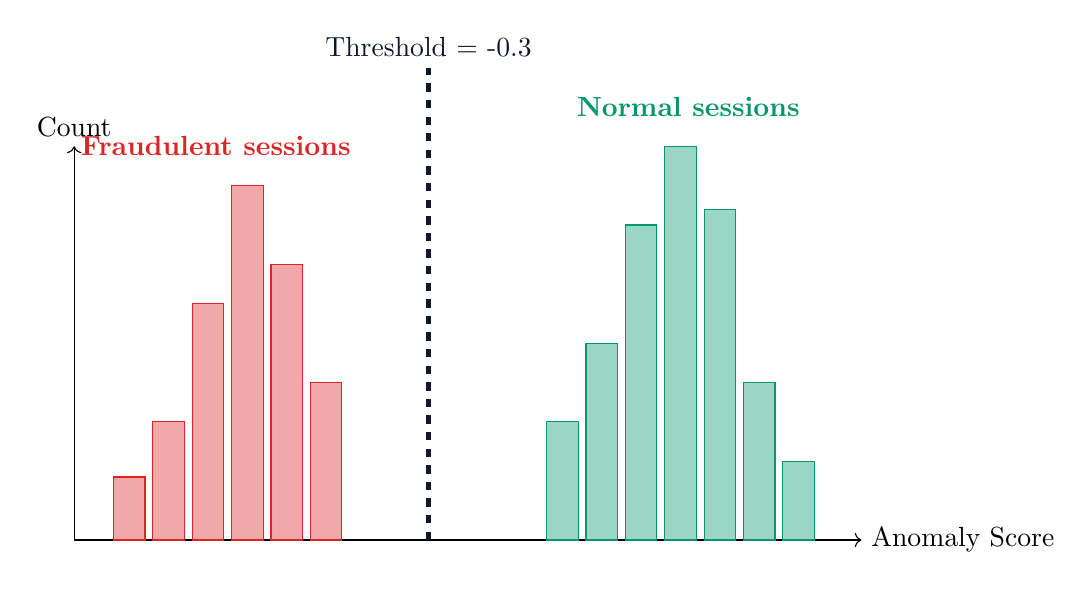
\begin{tikzpicture}
% High-performance manual bar chart to replace PGFPlots
\draw[->] (0,0) -- (10,0) node[right] {Anomaly Score};
\draw[->] (0,0) -- (0,5) node[above] {Count};

% Fraud Distribution (Red bars)
\foreach \x/\h in {0.5/0.8, 1.0/1.5, 1.5/3.0, 2.0/4.5, 2.5/3.5, 3.0/2.0} {
    \draw[certired, fill=certired!40] (\x,0) rectangle (\x+0.4,\h);
}
\node[certired] at (1.8,5.0) {\textbf{Fraudulent sessions}};

% Normal Distribution (Green bars)
\foreach \x/\h in {6.0/1.5, 6.5/2.5, 7.0/4.0, 7.5/5.0, 8.0/4.2, 8.5/2.0, 9.0/1.0} {
    \draw[certigreen, fill=certigreen!40] (\x,0) rectangle (\x+0.4,\h);
}
\node[certigreen] at (7.8,5.5) {\textbf{Normal sessions}};

% Threshold
\draw[dashed, ultra thick, certidark] (4.5,0) -- (4.5,6) node[above] {Threshold = -0.3};
\end{tikzpicture}
\caption{Distribution of anomaly scores with enforcement threshold}
\end{figure}

\subsection{Feature Table}
\begin{table}[H]
\centering
\caption{Behavioral features used for local anomaly scoring}
\begin{tabularx}{\textwidth}{>{\bfseries}lYY}
\toprule
Name & Normal Range & Fraud Indicator \\
\midrule
Active users & 5--60 & Sudden spikes beyond licensed capacity \\
Hour-of-day pattern & Business-hour dominant & High activity at abnormal hours \\
Unique machines (24h) & Stable tenant profile & Sharp fan-out across many hosts \\
API calls/minute & Predictable envelope & Burst amplification and scripted cadence \\
CPU percent & 10--75\% & Sustained high load from automation loops \\
Memory percent & 20--80\% & Unusual sustained pressure with license abuse \\
Process count & Environment baseline & Abrupt tooling/process injection patterns \\
GPU/discrete hint & Stable hardware signature & Unexpected hardware class shifts \\
\bottomrule
\end{tabularx}
\end{table}

\subsection{Offline-First Design}
Enforcement path: local detection $\rightarrow$ audit hash chain $\rightarrow$ vendor review at renewal/sync. No continuous cloud dependency is required; evidence accumulates locally and can be synchronized opportunistically.

% =================================================
% SECTION 8
% =================================================
\section{Complete Attack-Defense Matrix}

\begin{table}[H]
\centering
\caption{Attack-to-layer mapping across 14 scenarios}
\small
\begin{tabularx}{\textwidth}{c Y c Y Y}
\toprule
\textbf{ID} & \textbf{Attack Description} & \textbf{Layer} & \textbf{Detection Method} & \textbf{Result} \\
\midrule
\rowcolor{attackblue}
A1 & Edit signed field in license payload & L1 & Ed25519 signature verification fails & Rejected \\
\rowcolor{attackblue}
A2 & Replace \texttt{valid\_until} with future date & L1 & Signature mismatch on modified payload & Rejected \\
\rowcolor{attackgreen}
A3 & Copy license to a different machine & L2 & Hardware fingerprint mismatch & Rejected \\
\rowcolor{attackgreen}
A4 & Clone VM image to another host & L2/L3 & HW mismatch + DNA continuity break & Rejected \\
\rowcolor{attackgreen}
A5 & Snapshot rollback to older state & L3 & Monotonic counter regression & Rejected \\
\rowcolor{attackorange}
A6 & Patch executable branch around verify & L4 & Challenge-response integrity fails & Rejected \\
\rowcolor{attackorange}
A7 & Swap verifier response blob & L4 & HMAC challenge mismatch & Rejected \\
\rowcolor{attackred}
A8 & Attach debugger to runtime process & L5 & Anti-debug detectors + timing heuristics & Blocked / flagged \\
\rowcolor{attackred}
A9 & Single-step runtime to extract logic & L5 & Timing anomaly and debugger flags & Blocked / flagged \\
\rowcolor{attackpurple}
A10 & Kill watchdog/liveness process repeatedly & L6 & PoW heartbeat stale/chain invalid & Restricted mode \\
\rowcolor{attackblue}
A11 & Add \texttt{PREMIUM\_UNLOCK=true} in payload & L7 & Honeypot tripwire before full verify & Rejected \\
\rowcolor{attackpurple}
A12 & Share one license across many teams & L8 & Isolation Forest anomaly score crossing threshold & Flagged / blocked \\
\rowcolor{attackpurple}
A13 & Leak customer license on forums & L9 & Per-customer watermark attribution & Traceable source \\
\rowcolor{attackred}
A14 & Delete/modify audit evidence rows & L10 & Hash-chain verification failure & Tamper alert \\
\bottomrule
\end{tabularx}
\end{table}

% =================================================
% SECTION 9
% =================================================
\section{SDK Integration}

\subsection{Minimal Integration Snippet}
\begin{lstlisting}[language=Python,caption={Three-line host application integration}]
from certiguard.license_client import CertiGuardClient
result = CertiGuardClient(state_dir).verify_runtime(license_path=lic, public_key_path=pub)
assert result.ok, result.code
\end{lstlisting}

\subsection{Component Layout}
\begin{figure}[H]
\centering
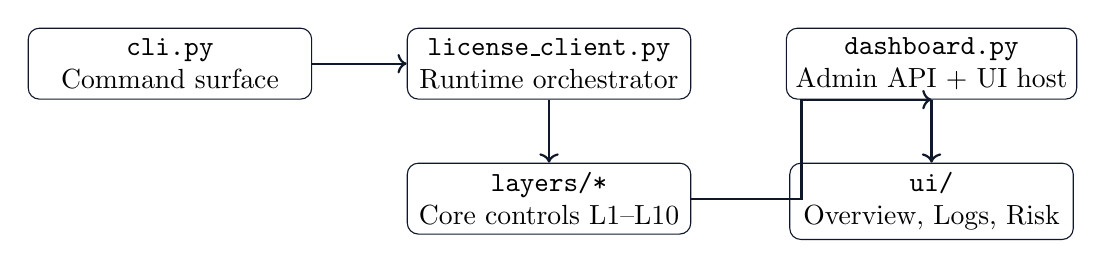
\begin{tikzpicture}[
  node distance=0.8cm and 1.2cm,
  box/.style={draw=certidark, rounded corners, fill=white, minimum width=3.6cm, minimum height=0.9cm, align=center},
  arr/.style={->, thick, certidark}
]
\node[box] (cli) {\texttt{cli.py}\\Command surface};
\node[box, right=of cli] (client) {\texttt{license\_client.py}\\Runtime orchestrator};
\node[box, below=of client] (layers) {\texttt{layers/*}\\Core controls L1--L10};
\node[box, right=of client] (dash) {\texttt{dashboard.py}\\Admin API + UI host};
\node[box, below=of dash] (ui) {\texttt{ui/}\\Overview, Logs, Risk};

\draw[arr] (cli) -- (client);
\draw[arr] (client) -- (layers);
\draw[arr] (layers.east) -- ++(1.4,0) |- (dash.south);
\draw[arr] (dash) -- (ui);
\end{tikzpicture}
\caption{CertiGuard SDK component interaction view}
\end{figure}

\subsection{Deployment Scenarios}
\begin{table}[H]
\centering
\caption{Deployment modes}
\begin{tabularx}{\textwidth}{>{\bfseries}lYc}
\toprule
Scenario & Active Layers & Internet Required \\
\midrule
Air-gapped & L1--L10 (no external online ping dependency) & NO \\
Standard enterprise & All layers + optional sync at renewal & NO \\
Trial copy & L1 + L7 (lightweight policy mode) & NO \\
\bottomrule
\end{tabularx}
\end{table}

% =================================================
% SECTION 10
% =================================================
\section{References}

\begin{enumerate}[label={[\arabic*]}]
\item D. J. Bernstein, N. Duif, T. Lange, P. Schwabe, and B.-Y. Yang, ``High-speed high-security signatures,'' \emph{Journal of Cryptographic Engineering}, 2011.
\item IETF, ``RFC 8032: Edwards-Curve Digital Signature Algorithm (EdDSA),'' 2017.
\item J. Brendel, C. Cremers, and D. Jackson, ``A formal treatment of Ed25519 signature security,'' in \emph{IEEE Symposium on Security and Privacy}, 2021.
\item F. T. Liu, K. M. Ting, and Z.-H. Zhou, ``Isolation Forest,'' in \emph{IEEE International Conference on Data Mining (ICDM)}, 2008.
\item B. De Sutter, A. Slowinska, and S. Schrittwieser, ``Software protection methodologies: State of the art and open challenges,'' \emph{ACM Computing Surveys}, 2024.
\item S. Chow, P. A. Eisen, H. Johnson, and P. C. van Oorschot, ``White-box cryptography and implementation attacks,'' in \emph{SAC}, 2002.
\item National Security Agency, ``Trusted Platform Module (TPM) Use Cases and Deployment Guidance,'' Technical Report, 2024.
\item S. Nakamoto, ``Bitcoin: A Peer-to-Peer Electronic Cash System,'' 2008.
\end{enumerate}

\begin{tcolorbox}[certicallout,title=\textbf{Final Note}]
This architecture is intentionally offline-first: it prioritizes local enforceability, cryptographic authenticity, and forensic continuity while still enabling periodic vendor-side review through synchronized or transferred audit evidence.
\end{tcolorbox}

\end{document}
